\documentclass{beamer}
\usepackage[swedish]{babel}
\usepackage[utf8]{inputenc}
\usepackage[utf8]{inputenc}
\usepackage{amsmath}
\usepackage{amssymb}
\usepackage{amsthm}
\usepackage{graphicx}

\uselanguage{swedish}
\languagepath{swedish}
\deftranslation[to=swedish]{Theorem}{Sats}
\deftranslation[to=swedish]{theorem}{sats}
\deftranslation[to=swedish]{Example}{Exempel}
\deftranslation[to=swedish]{example}{exempel}




\usetheme{Warsaw}

\title[Algoritmer och komplexitet inom algebraisk geometri]{
	Algoritmer och komplexitet inom \\
	kommutativ algebra \& algebraisk geometri \\[20pt]
	\large Omparametrisering av kurvor, semigrupper, \\
	implicit notation \& multiplicitetsföljder}

\author[Peter Waher]{Peter Waher \\[10pt]
	\texttt{peterwaher@hotmail.com}\\
	\texttt{https://github.com/PeterWaher/Algebraiska\_kurvor}}

\begin{document}

\begin{frame}
	\titlepage
\end{frame}

\begin{frame}
	\frametitle{Outline}
	\tableofcontents[pausesections]
\end{frame}





\section{Plana algebraiska kurvor}
\subsection{Introduktion - kurvor}


\begin{frame}
	\frametitle{Plana algebraiska kurvor}
	\begin{enumerate}
		\item<1-> Plana algebraiska kurvor
		\begin{enumerate}
			\item<2-> Introduktion
			\item<3-> Omparametrisering
		\end{enumerate}
	\end{enumerate}
\end{frame}

\begin{frame}
\frametitle{Vad är en plan kurva?}
\begin{Definition}
	En \textbf{plan kurva} $C$ är en delmängd i $\mathbb{C}^2$ sådan att det finns två kontinuerliga funktioner $f : \mathbb{C} \rightarrow \mathbb{C}$ och 
	$g : \mathbb{C} \rightarrow \mathbb{C}$ sådana att $C = \left\{\left(f(t), g(t)\right) : t \in \mathbb{C}\right\}$. $(f, g)$ är en \textbf{parametrisering} av $C$. Om $C$ kan parametriseras av två analytiska funktioner $f$ och $g$ kallas $C$ \textbf{analytisk}. Om den kan parametriseras av två polynom kallas $C$ för \textbf{algebraisk}. Om den kan parametriseras av två formella potensserier kallas $C$ \textbf{algebroid}.
\end{Definition}
\end{frame}

\begin{frame}
	\frametitle{Kurvor i det Euklidiska planet}
	Traditionellt har man ofta studerat plana kurvor i det \emph{Euklidiska planet}. I detta fall är kurvan parametriserad av reellvärda funktioner $f : \mathbb{R} \rightarrow \mathbb{R}$ och 
	$g : \mathbb{R} \rightarrow \mathbb{R}$.
	
  	\begin{example}
		\begin{columns}[onlytextwidth]
			\begin{column}{0.55\textwidth}
				\[C(t)=(t^2,t^3+t^7)\]\\[10pt]
				\scriptsize Not: För att förenkla notationen kan vi identifiera kurvan $C$ med en viss parametrisering $(f, g)$, även om parametriseringen inte är unik. Detta görs enklast genom att identifiera kurvan med funktionen $C : \mathbb{C} \rightarrow \mathbb{C}^2$, $C(t) = \left(f(t), g(t)\right)$. Notera dock att kurvan som sådan och en av dess parametriseringar är två olika objekt.
			\end{column}
			\begin{column}{0.45\textwidth}
				\begin{center}
				\includegraphics[scale=0.3]{Export/blowupex1_1.png}
				\end{center}
			\end{column}
		\end{columns}
  	\end{example}
\end{frame}


\begin{frame}
	\frametitle{Förenklingar}
	Förenklingar vi kan göra om vi studerar en plan kurva lokalt:
	
	\begin{enumerate}
		\item<1-> Tillräckligt att studera \emph{algebraiska} kurvor:
		\begin{enumerate}
			\item<2-> Analytiska funktioner kan skrivas som formella potensserier kring den punkt vi studerar.
			\item<3-> Formella potensserier kan approximeras av polynom med önskad noggrannhet.
		\end{enumerate}
		\item<4-> Kurvan går genom \emph{origo}: $C(0) = \mathbf{0}$
	\end{enumerate}
\end{frame}

\begin{frame}
	\frametitle{Reguljära och singulära kurvor}
\begin{Definition}
	Om en kurva $C$ har en parametrisering $(f, g)$ sådan att $f'(0) \neq 0$ eller $g'(0) \neq 0$ kallas kurvan \textbf{reguljär}. Annars kallas kurvan \textbf{singulär}.
\end{Definition}

\vspace{20pt}
\scriptsize Not: Bara för att $f'(0) = 0$ och $g'(0) = 0$ i en parametrisering $(f, g)$ av en kurva $C$, betyder inte det att kurvan är singulär. Det kan ju finnas en parametrisering av samma kurva där någon av derivatorna är nollskilda. Exempelvis är $(t^3, t^3)$ och $(t, t)$ två olika parametriseringar av samma kurva. I det första exemplet är derivatorna $0$ i origo medan de i det andra exemplet båda är nollskilda.
\end{frame}

\begin{frame}
	\frametitle{Ordning och grad}
\begin{Definition}
	\textbf{Ordningen} av ett polynom eller en potensserie $f(t) =
	\sum a_i t^i \neq 0$ är det minsta heltalet $k$ sådant att koefficienten $a_k$ är nollskild, och skrivs $\mathbf{o}(f)$. \textbf{Graden} for motsvarande polynom är det största heltalet $k$ sådant att koefficienten $a_k$ inte är noll, och skrivs $\deg(f)$.
\end{Definition}
\end{frame}

\subsection{Omparametrisering}

\begin{frame}
	\frametitle{Varför omparametrisera?}
	\begin{enumerate}
		\item För utritande av kurvor spelar parametriseringen inte så stor roll.
		
		\item Vill man beräkna $y(x) = g(f^{-1}(x))$ eller $x(y) = f(g^{-1}(y))$, står man genast inför en mängd problem.
	\end{enumerate}
\end{frame}

\begin{frame}
	\frametitle{Omparametrisering av kurvor}
\begin{Theorem}
	Om $C = C(t) = \left(f(t), g(t)\right)$ är en komplex analytisk, algebroid eller algebraisk kurva, samt att $f(0) = g(0) = 0$, kan kurvan $C$ omparametriseras på formen $C^*(t) = \left(\pm t^n, g^*(t)\right)$ eller på formen $C^*(t) = \left(f^*(t), \pm t^n \right)$ i ett område kring $t = 0$, där $f(t)$ och $g(t)$ är formella potensserier. Dessutom gäller att $\mathbf{o}\left(f^*\right) \geq n$ eller att $\mathbf{o}\left(g^*\right) \geq n$. Om $f(t)$ och $g(t)$ är reellvärda, kan också omparametriseringen göras reellvärd.
\end{Theorem}

\vspace{20pt}
\scriptsize Not: Från \emph{Weierstrass Preparation Theorem} kan man få att en sådan omparametrisering existerar. Dock presenteras inte en metod över hur en sådan omparametrisering kan tas fram.
\end{frame}

\begin{frame}
	\frametitle{Översikt bevis}
	Beviset av satsen går igenom följande steg:
	
	\begin{enumerate}
		\item<1-> Vi skapar en omparametrisering via komposition med $\phi(t)$:
		\[C^*(t) = (f^*(t), g^*(t)) = (f(\phi(t)), g(\phi(t)))\]
		
		\item<2-> Vi väljer $\phi(t)$ sådan att:
		\begin{enumerate}
			\item<3-> Analytisk kring $t = 0$.
			
			\item<4-> $\phi(0)=0$
			
			\item<5-> $\mathbf{o}(\phi)=1 \Longrightarrow \mathbf{o}(f(\phi))=\mathbf{o}(f) \wedge \mathbf{o}(g(\phi))=\mathbf{o}(g)$
			
			\item<6-> $\phi(t), f(t), g(t)$ reellvärda $\Longrightarrow$ $C^*(t)$ reellvärd.
			
		\end{enumerate}
		
		\item<7-> Med början i $a_1$ (som har $n$ lösningar), löses koefficienterna $a_i$ ut ur $\phi(t)=\sum_{k=1}^{\infty}a_k t^k$ för att uppfylla ovanstående.
		
		\item<8-> Finns precis en lösning i det generella fallet som uppfyller ovanstående, samt satsens, krav.
		
	\end{enumerate}
\end{frame}

\begin{frame}
	\frametitle{\texttt{Reparametrize()}}

\begin{semiverbatim}
Reparametrize := proc(x, y, Variable, t0 , MaxDegree,

\qquad Branch, AllowNegation)
\end{semiverbatim}
	
	\begin{enumerate}
		\item<1-> Algoritm som omparametriserar en algebraisk kurva med given noggrannhet.
		
		\item<2-> Maple-kod finns i \texttt{https://github.com/PeterWaher/\\
			\qquad Algebraiska\_kurvor/blob/master/kurvor.mw}
		
		\item<3-> Text-version finns i
		\texttt{https://github.com/PeterWaher/\\
			\qquad Algebraiska\_kurvor/blob/master/Functions/\\
			\qquad Reparametrize.txt} 
	\end{enumerate}
\end{frame}




\begin{frame}
	\frametitle{Reparametrize - exempel 1 (1/4)}
	
  	\begin{example}
  		Kurvan $(t^2+t^3,t^5+t^6)$ har en singularitet i $t = 0$. Dessutom passerar kurvan genom origo då $t = -1$.
  		
		\begin{center}
			\includegraphics[scale=0.35]{Export/kurvorplot2d1_0.png}
		\end{center}
  	\end{example}
\end{frame}
  		
\begin{frame}
	\frametitle{Reparametrize - exempel 1 (2/4)}
	
	\begin{example}
  		Först ber vi Maple att parametrisera om kurvan kring $t = 0$:
  		
		\begin{semiverbatim}
		> Reparametrize(t\^{}3+t\^{}2,t\^{}6+t\^{}5,t,0,10,0,false);
		
		
		Elapsed Time: 0.016 s.
		\end{semiverbatim}
				 
		 \[\left[{t}^{2},{t}^{5}-3/2\,{t}^{6}+{\frac {21\,{t}^{7}}{8}}-5\,{t}^{8}+{\frac {1287\,{t}^{9}}{128}}-21\,{t}^{10}\right]\]
  	\end{example}
\end{frame}

\begin{frame}
	\frametitle{Reparametrize - exempel 1 (3/4)}
	
	\begin{example}
		Därefter vill vi ha en omparametrisering kring $t = -1$:

\begin{semiverbatim}
> Reparametrize(t\^{}3+t\^{}2, t\^{}6+t\^{}5, t, -1, 10,

\qquad 0, false);


Elapsed Time: 0.016 s.
\end{semiverbatim}		
		\[\left[t,163438\,{t}^{10}+29070\,{t}^{9}+5304\,{t}^{8}+1001\,{t}^{7}+198\,{t}^{6}+42\,{t}^{5}+\right.\]
		\[\left.+10\,{t}^{4}+3\,{t}^{3}+3\,{t}^{2}-t\right]\]
	\end{example}
\end{frame}

\begin{frame}
	\frametitle{Reparametrize - exempel 1 (4/4)}
	
	\begin{example}
	Nedan kurvan $C(t)=(t^2+t^3,t^5+t^6)$, med omparametriseringarna kring $t=0$ och $t=-1$.
	
		\begin{center}
			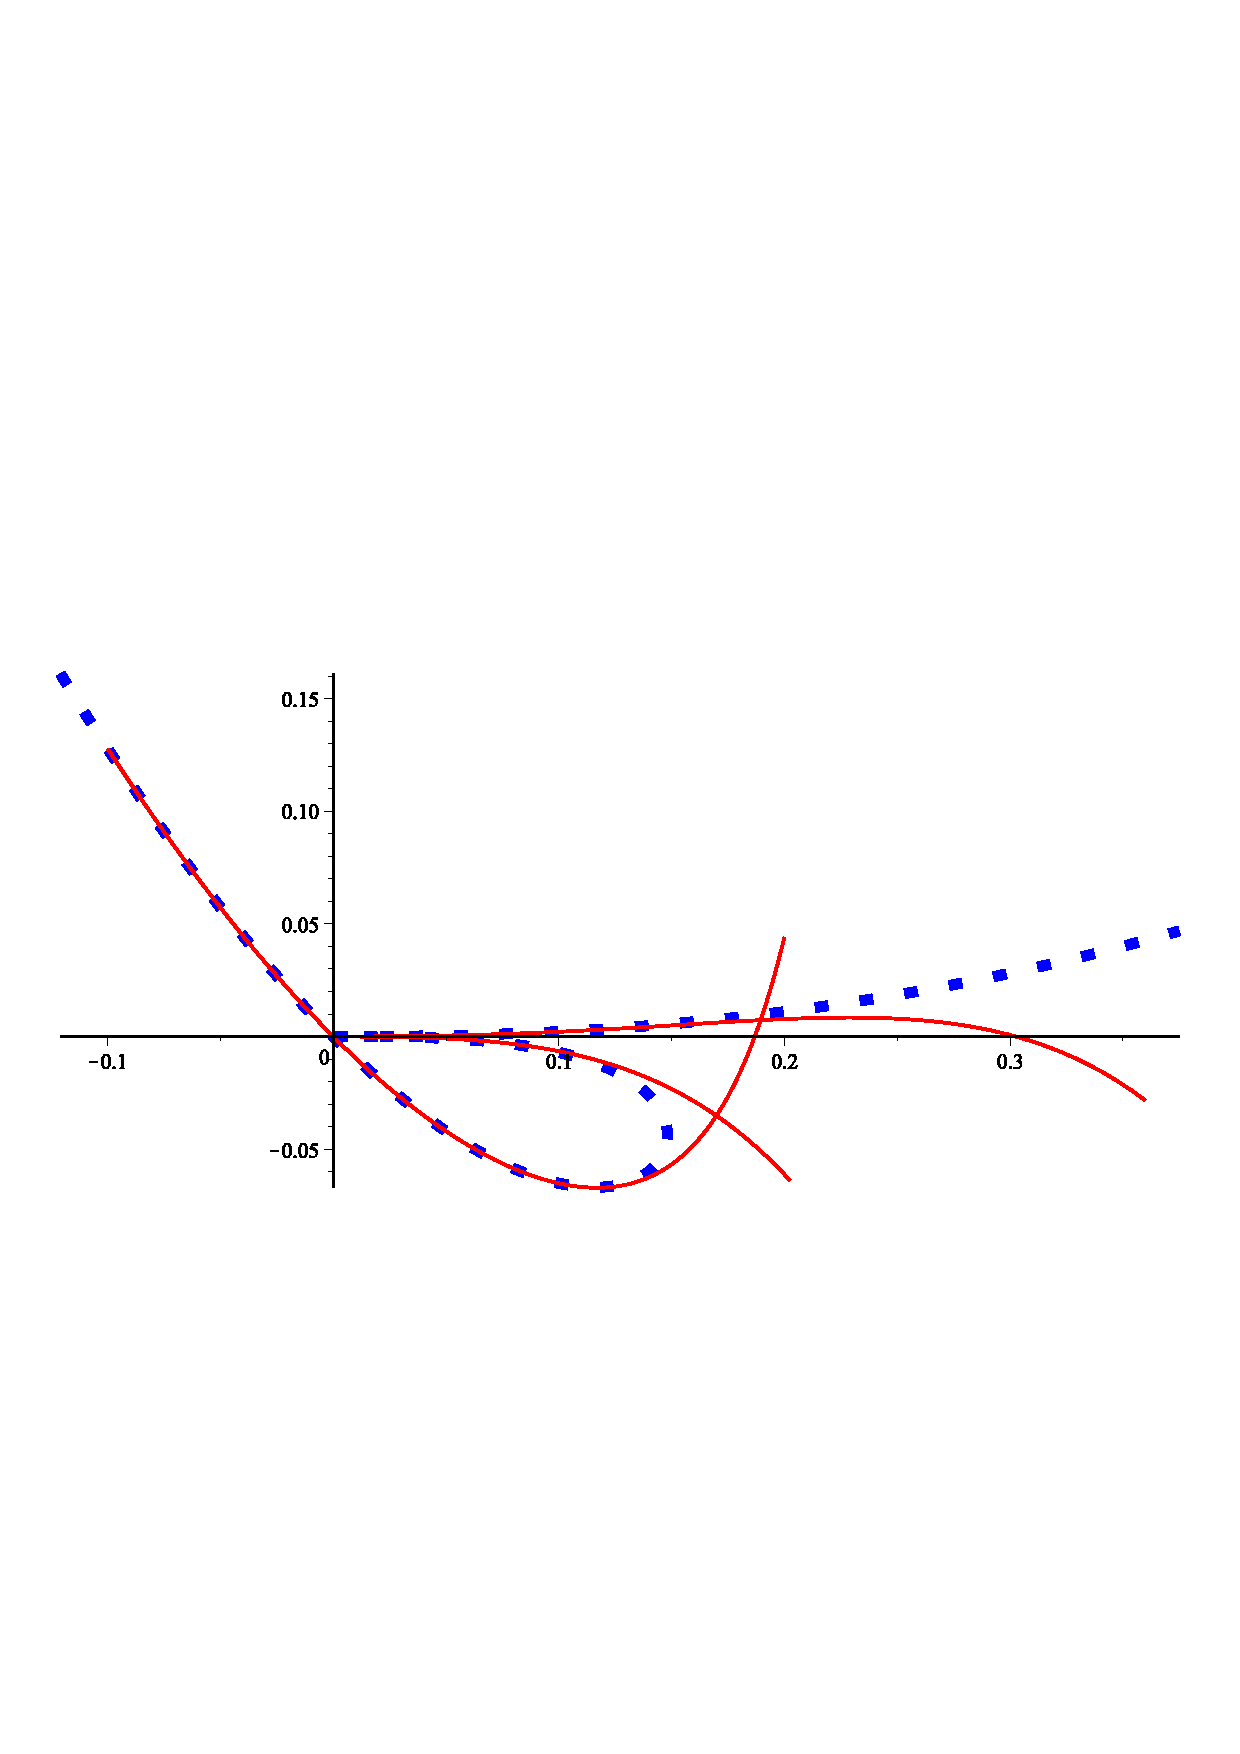
\includegraphics[scale=0.35]{Export/kurvorplot2d1.png}
		\end{center}
	\end{example}
\end{frame}






\begin{frame}
	\frametitle{Reparametrize - exempel 2 (1/6)}
	
	\begin{example}
		Ellipsen $\left(3 \sin(t), 2 \cos(t)\right)$ är reguljär, men vi kan parametrisera om kurvan ändå för att illustrera axelbyte. 
  		
  		\begin{center}
  			\includegraphics[scale=0.35]{Export/kurvorplot2d2_0.png}
  		\end{center}
  	\end{example}
  \end{frame}
  
  \begin{frame}
  	\frametitle{Reparametrize - exempel 2 (2/6)}
  	
  	\begin{example}
		Första omparametriseringen gör vi kring $t=0$:

		\begin{semiverbatim}
			> Reparametrize(3*sin(t),2*cos(t),t,0,10,0,false);
			
			
			Elapsed Time: 0.015 s.
		\end{semiverbatim}
		
		\[\left[t,2-1/9\,{t}^{2}-{\frac {{t}^{4}}{324}}-{\frac {{t}^{6}}{5832}}-{\frac {5\,{t}^{8}}{419904}}-{\frac {7\,{t}^{10}}{7558272}}\right]\]
	\end{example}
\end{frame}

\begin{frame}
	\frametitle{Reparametrize - exempel 2 (3/6)}
	
	\begin{example}
		Andra omparametriseringen gör vi kring $t=\pi$:
		
		\begin{semiverbatim}
			> Reparametrize(3*sin(t),2*cos(t),t,Pi,10,0,false);
			
			
			Elapsed Time: 0.016 s.
		\end{semiverbatim}
		
		\[\left[t,-2+1/9\,{t}^{2}+{\frac {{t}^{4}}{324}}+{\frac {{t}^{6}}{5832}}+{\frac {5\,{t}^{8}}{419904}}+{\frac {7\,{t}^{10}}{7558272}}\right]\]
	\end{example}
\end{frame}

\begin{frame}
	\frametitle{Reparametrize - exempel 2 (4/6)}
	
	\begin{example}
		Tredje omparametriseringen gör vi kring $t=\frac{\pi}{2}$. Notera hur omparametriseringarna skiljer från $t=0$ och $t=\pi$, jämfört med $t=\pm \frac{\pi}{2}:$
		
		\begin{semiverbatim}
			> Reparametrize(3*sin(t),2*cos(t),t,(1/2)*Pi,

			\qquad 10,0,false);
			
			
			Elapsed Time: 0.016 s.
		\end{semiverbatim}
		
		\[\left[3-3/8\,{t}^{2}-{\frac {3\,{t}^{4}}{128}}-{\frac {3\,{t}^{6}}{1024}}-{\frac {15\,{t}^{8}}{32768}}-{\frac {21\,{t}^{10}}{262144}},t\right]\]
	\end{example}
\end{frame}

\begin{frame}
	\frametitle{Reparametrize - exempel 2 (5/6)}
	
	\begin{example}
		Fjärde omparametriseringen gör vi kring $t=-\frac{\pi}{2}$:
		
		\begin{semiverbatim}
			> Reparametrize(3*sin(t),2*cos(t),t,-(1/2)*Pi,
			
			\qquad 10,0,false);
			
			
			Elapsed Time: 0.015 s.
		\end{semiverbatim}
		
		\[\left[-3+3/8\,{t}^{2}+{\frac {3\,{t}^{4}}{128}}+{\frac {3\,{t}^{6}}{1024}}+{\frac {15\,{t}^{8}}{32768}}+{\frac {21\,{t}^{10}}{262144}},t\right]\]
	\end{example}
\end{frame}

\begin{frame}
	\frametitle{Reparametrize - exempel 2 (6/6)}
	
	\begin{example}
		Nedan kurvan $C(t)=(3\sin(t),2\cos(t))$, med de fyra omparametriseringarna kring $t=0$, $t=\pi$ och $t=\pm \frac{\pi}{2}$:
		
		\begin{center}
			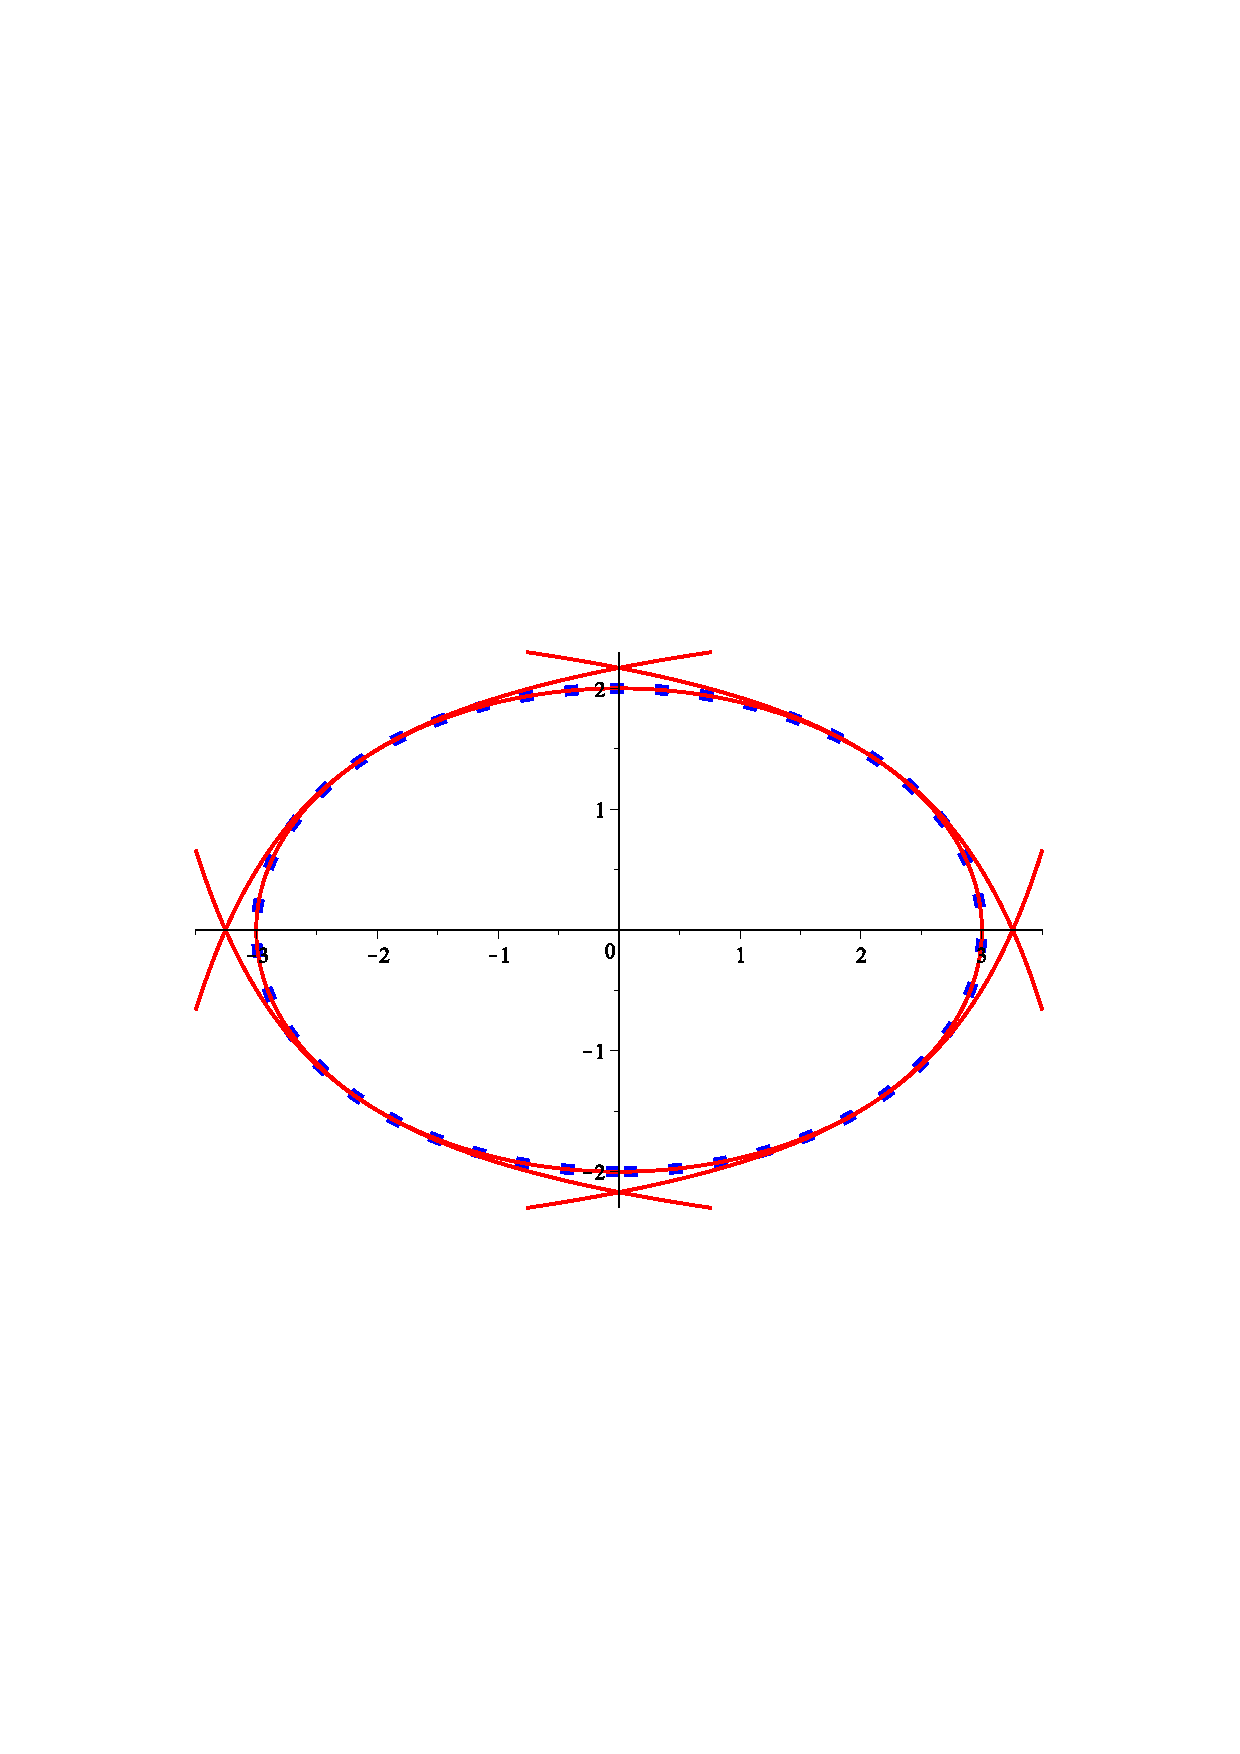
\includegraphics[scale=0.35]{Export/kurvorplot2d2.png}
		\end{center}
	\end{example}
\end{frame}






\begin{frame}
	\frametitle{Reparametrize - exempel 3 (1/5)}
	
	\begin{example}
		Kurvan $\left(t^3(t - 1)^3(t + 1)^3,t^5(t - 1)^2(t + 1)^2\right)$ har singulariteter i $t = 0, 1, -1$ av ordningar 2, 1, 1 respektive.
  		
  		\begin{center}
  			\includegraphics[scale=0.35]{Export/kurvorplot2d3_0.png}
  		\end{center}
  	\end{example}
  \end{frame}
  
  \begin{frame}
  	\frametitle{Reparametrize - exempel 3 (2/5)}
  	
  	\begin{example}
		Vi analyserar hur omparametriseringarna uppför sig i dessa tre singulariteter. Första omparametriseringen gör vi kring $t=0$:

		\begin{semiverbatim}
			> Reparametrize(t\^{}3*(t-1)\^{}3*(t+1)\^{}3,

			\qquad t\^{}5*(t-1)\^{}2*(t+1)\^{}2,t,0,15,0, false);
			
			
			Elapsed Time: 0.031 s.
		\end{semiverbatim}
		
		\[\left[{t}^{3},-1428\,{t}^{15}-273\,{t}^{13}-55\,{t}^{11}-12\,{t}^{9}-3\,{t}^{7}-{t}^{5}\right]\]
	\end{example}
\end{frame}

\begin{frame}
	\frametitle{Reparametrize - exempel 3 (3/5)}
	
	\begin{example}
		Därefter kring $t=1$:
		
		\begin{semiverbatim}
			> Reparametrize(t\^{}3*(t-1)\^{}3*(t+1)\^{}3,
			
			\qquad t\^{}5*(t-1)\^{}2*(t+1)\^{}2,t,1,15,0,false);
			
			
			Elapsed Time: 0.063 s.
		\end{semiverbatim}
		
		\[\begin{array}{l}
		\left[1/2\, \sqrt{4}{t}^{3}-9/4\,{t}^{4}+{\frac {207\, \sqrt{4}{t}^{5}}{64}}-21\,{t}^{6}+{\frac {150183\, \sqrt{4}{t}^{7}}{4096}}\right. \\
		\mbox{}-{\frac {137655\,{t}^{8}}{512}}+{\frac {66893079\, \sqrt{4}{t}^{9}}{131072}}-3978\,{t}^{10}+{\frac {132735945771\, \sqrt{4}{t}^{11}}{16777216}}\\
		\mbox{}-{\frac {8385901667\,{t}^{12}}{131072}}+{\frac {70379121262905\, \sqrt{4}{t}^{13}}{536870912}}\\
		\left.\mbox{}-{\frac {4345965\,{t}^{14}}{4}}+{\frac {78087826643607459\, \sqrt{4}{t}^{15}}{34359738368}},{t}^{2}\right]
		\end{array}\]
	\end{example}
\end{frame}

\begin{frame}
	\frametitle{Reparametrize - exempel 3 (4/5)}
	
	\begin{example}
		Och sist kring $t=-1$:
		
		\begin{semiverbatim}
			> Reparametrize(t\^{}3*(t-1)\^{}3*(t+1)\^{}3,
			
			\qquad t\^{}5*(t-1)\^{}2*(t+1)\^{}2,t,-1,15,0,true);
			
			
			Elapsed Time: 0.047 s.
		\end{semiverbatim}
		
		\[\begin{array}{l}
		\left[1/2\, \sqrt{4}{t}^{3}+9/4\,{t}^{4}+{\frac {207\, \sqrt{4}{t}^{5}}{64}}+21\,{t}^{6}+{\frac {150183\, \sqrt{4}{t}^{7}}{4096}}\right.\\
		\mbox{}+{\frac {137655\,{t}^{8}}{512}}+{\frac {66893079\, \sqrt{4}{t}^{9}}{131072}}+3978\,{t}^{10}+{\frac {132735945771\, \sqrt{4}{t}^{11}}{16777216}}\\
		\mbox{}+{\frac {8385901667\,{t}^{12}}{131072}}+{\frac {70379121262905\, \sqrt{4}{t}^{13}}{536870912}}\\
		\left.\mbox{}+{\frac {4345965\,{t}^{14}}{4}}+{\frac {78087826643607459\, \sqrt{4}{t}^{15}}{34359738368}},-{t}^{2}\right]
		\end{array}\]
	\end{example}
\end{frame}

\begin{frame}
	\frametitle{Reparametrize - exempel 3 (5/5)}
	
	\begin{example}
		Ritar vi sedan ut originalparametriseringen av kurvan tillsammans med de tre omparametriseringarna får vi följande intressanta bild:

		\begin{center}
			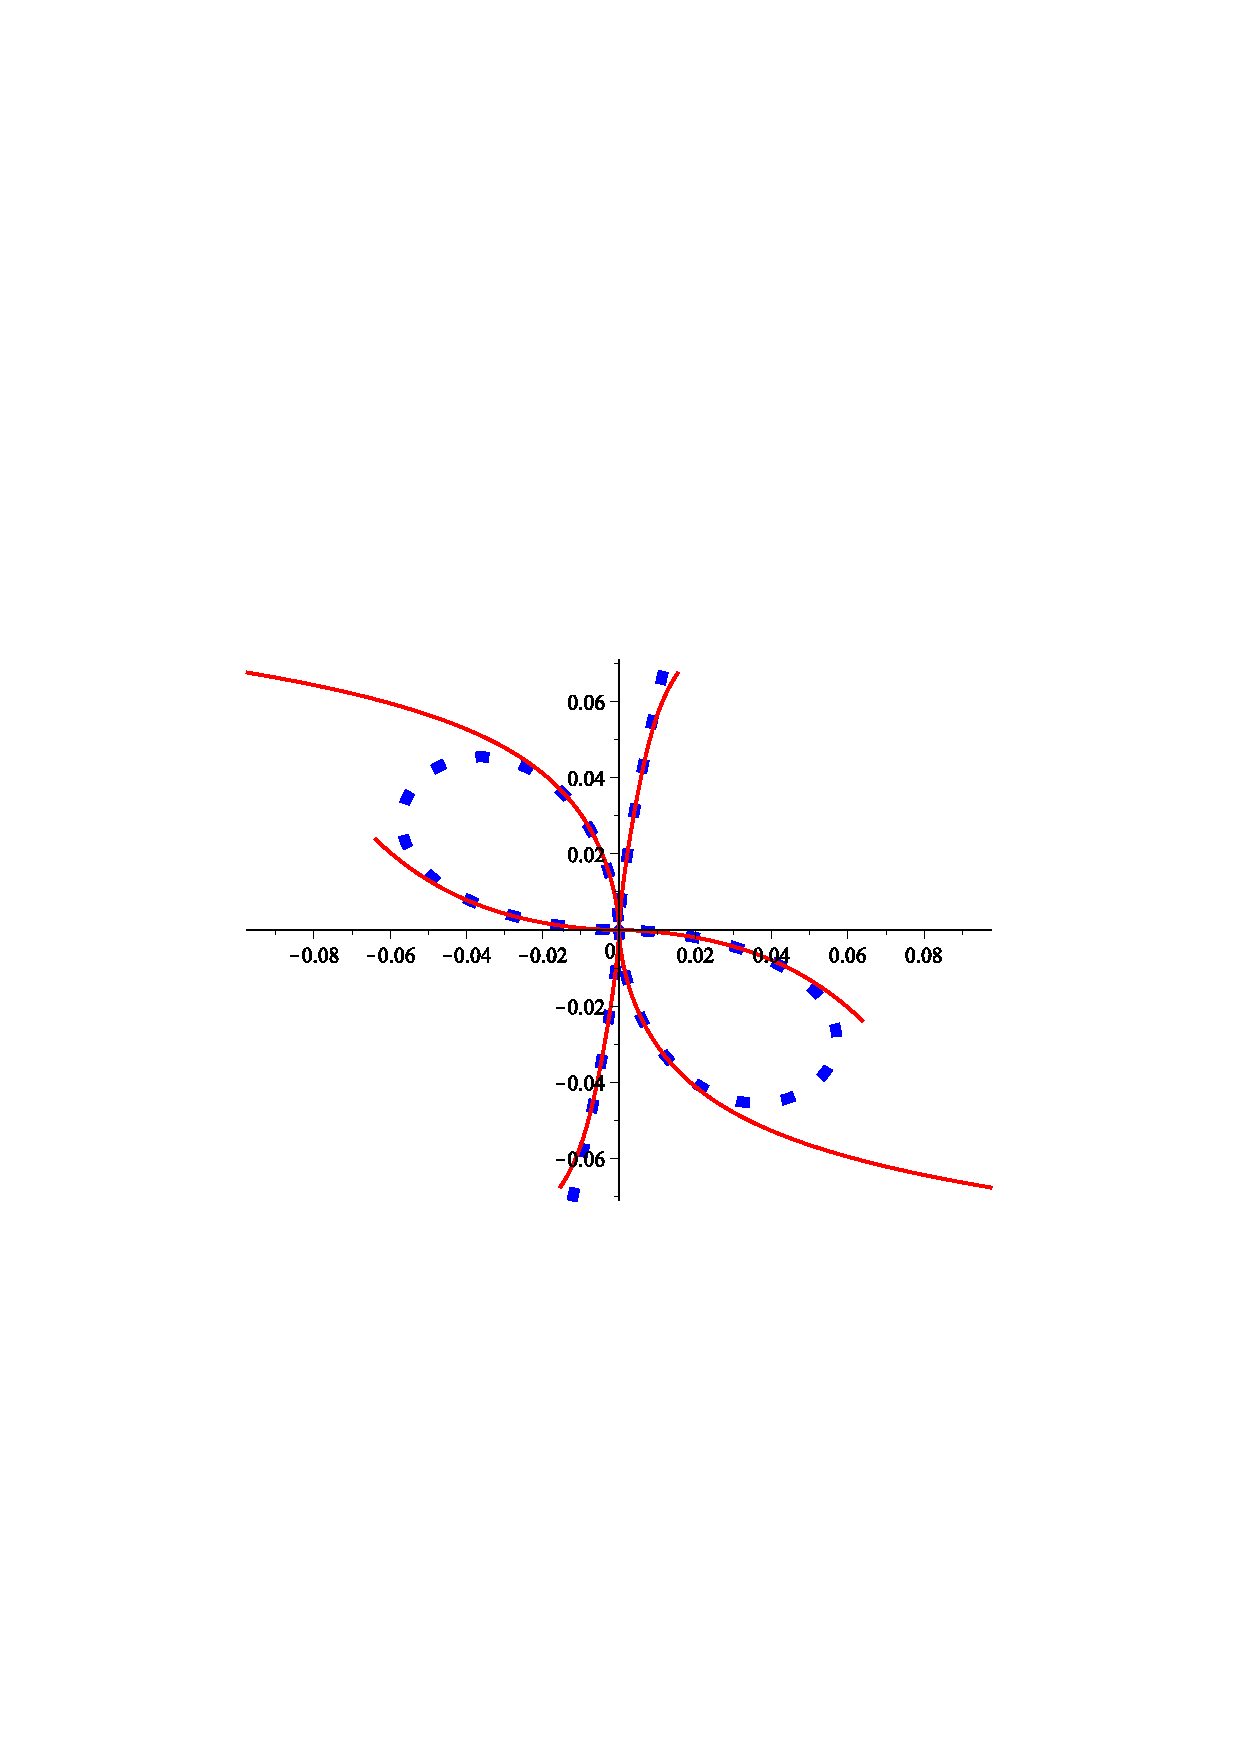
\includegraphics[scale=0.35]{Export/kurvorplot2d3.png}
		\end{center}
	\end{example}
\end{frame}








\section{Semigrupper}
\subsection{Introduktion - semigrupper}


\begin{frame}
	\frametitle{Semigrupper}
	\begin{enumerate}
		\setcounter{enumi}{1}
		\item<1-> Semigrupper
		\begin{enumerate}
			\item<2-> Modulär aritmetik
			\item<3-> Semigrupper
			\item<4-> Numeriska semigrupper
			\item<5-> Konduktören
			\item<6-> $\mathbb{C}[t]$ och dess delringar
			\item<7-> Semigrupper för $\mathbb{C}[p_1,\ldots,p_n]$
		\end{enumerate}
	\end{enumerate}
\end{frame}


\begin{frame}
	\frametitle{Modulär aritmetik}
\begin{Definition}
	Heltalen $m \in \mathbb{Z}^+$ och $n \in \mathbb{Z}^+$ sägs vara \textbf{relativt prima} om $m \geq 2$, $n \geq 2$ samt $p \mid m \wedge p \mid n \Longrightarrow p = 1$.
\end{Definition}
\uncover<2->{\begin{Lemma}
	Om $m$ och $n$ är relativt prima och $0 < a < m$ gäller att $[a \cdot n]_m \neq 0$.
	\end{Lemma}}
\uncover<3->{\begin{Lemma}
		Om $m$ och $n$ är relativt prima och $0 < a, b < m$ gäller:
		\[[a \cdot n]_m = [b \cdot n]_m \Longleftrightarrow a = b\]
	\end{Lemma}}
\end{frame}

\begin{frame}
	\frametitle{Semigrupper}
\begin{Definition}
	För en \textbf{semigrupp} $G$, med den implicit definierade binära operatorn $+$ gäller:
	\[a \in G \wedge b \in G \Longrightarrow (a + b) \in G\]
	\[(a+b)+c = a+(b+c)\]
\end{Definition}
\end{frame}

\begin{frame}
	\frametitle{Generatorer av semigrupp}
\begin{Definition}
	En serie tal $n_1, \ldots, n_k$ \textbf{genererar} semigruppen $G$ om
	\[G = \left\{\sum_{a_i\neq 0} a_i \cdot n_i : a_i \in \mathbb{N}\text{, inte alla $a_i=0$}\right\}\]
	Detta skrivs även $G = \left<n_1, \ldots, n_k \right>$.
\end{Definition}

\vspace{20pt}
\scriptsize Not: Notera att med multiplikation med ett positivt heltal inom en semigrupp avses repetitiv användning av additionsoperatorn.
\end{frame}

\begin{frame}
	\frametitle{Konduktören för $\left<m,n\right>$ ($m, n$ relativt prima)}
\begin{Theorem}
	Om $m$ och $n$ är relativt prima innehåller semigruppen $G = \left<m, n\right>$ alla tal större än eller lika med $c = (m - 1)(n - 1)$, men inte talet $c - 1$.
\end{Theorem}

\uncover<2->{Översikt av bevis:}
\begin{enumerate}
	\item<3-> $\mathbb{Z}_m = \left<[n]_m\right>$.
	\item<4-> Antag att $m<n$.
	\item<5-> Uppdelning av $\mathbb{N}$ i segment om $m$ tal vardera.
	\item<6-> Stryk alla tal i $[0]_m$, därefter $[n]_m$, $[2n]_m$, \ldots, $\left[(m-1)n\right]_m$.
	\item<7-> Alla tal större än eller lika med $(m-1)n$ ur $\mathbb{N}$
	\item<8-> Det högsta ostrukna talet, är således $(m - 1)n - m$.
\end{enumerate}
\end{frame}

\begin{frame}
	\frametitle{Numerisk semigrupp}
\begin{Definition}
	En \textbf{numerisk semigrupp} $G$ är en speciell form av semigrupp, där även följande villkor gäller:
	\[
	\begin{array}{rcl}
	G & \subseteq & \mathbb{N} \\
	\left\| \mathbb{N} \setminus G \right\| & < & \infty \\
	\end{array}\]
\end{Definition}

\uncover<2->{\begin{Lemma}
		$G = \left<m, n\right>$ där $m$ och $n$ är relativt prima, är en numerisk semigrupp.
	\end{Lemma}
	}
\end{frame}

\begin{frame}
	\frametitle{Konduktör}
\begin{Definition}
	I varje numerisk semigrupp $G$ finns det ett tal $c_G$ sådant att följande villkor uppfylls:
	\[\begin{array}{rcl}
	c_G & \in & G \\
	n > c_G & \Longrightarrow & n \in G \\
	c_G - 1 & \notin & G \\
	\end{array}\]
	$c_G$ kallas för \textbf{konduktören} för $G$.
\end{Definition}
\uncover<2->{$c=(m-1)(n-1)$ där $m$ och $n$ är relativt prima, är konduktör för den numeriska semigruppen $G = \left<m, n\right>$.}
\end{frame}

\begin{frame}
	\frametitle{$\gcd(n_1, \ldots, n_k) = 1$}
\begin{Theorem}
	Om semigruppen $G = \left<n_1, \ldots, n_k\right>$ är numerisk så är den största gemensamma delaren av talen $\gcd(n_1, \ldots, n_k) = 1$.
\end{Theorem}

\uncover<2->{Översikt av trivialt bevis:}
\begin{enumerate}
	\item<3-> $\gcd(G)=\gcd(n_1,\ldots,n_k)=d$.
	\item<4-> $d>1 \Longrightarrow \left\|\mathbb{N} \setminus G \right\| = \infty$
\end{enumerate}
\end{frame}

\begin{frame}
	\frametitle{Minimalt generatorsystem}
\begin{Theorem}
	För varje numerisk semigrupp $G$ finns ett minimalt generatorsystem $n_1, \ldots, n_k$, sådant att $G = \left<n_1, \ldots, n_k\right>$. Detta system är unikt för $G$.
\end{Theorem}

\uncover<2->{Översikt av bevis:}
\begin{enumerate}
	\item<3-> Ändlig mängd tal i $G$ som genererar semigruppen.
	\item<4-> $\widehat{M}$ mängden av alla ändliga mängder av generatorer.
	\item<5-> $\widehat{M}' = \{ \left\|M\right\| : M \in \widehat{M}\}$
	\item<6-> $k = \inf \widehat{M}'$ existerar.
	\item<7-> $\exists M_- \in \widehat{M} : \left\|M_-\right\|=k$
	\item<8-> $N_- \in \widehat{M} \wedge \left\|N_-\right\|=k \Longrightarrow N_- = M_-$
\end{enumerate}\end{frame}

\subsection{Beräkning av konduktören}

\begin{frame}
	\frametitle{$\gcd(\left\{n_i\right\})=1 \Longrightarrow \left<\left\{n_i\right\}\right> \text{ numerisk}$}
\begin{Theorem}
	Om $n_1, \ldots, n_k$ är heltal sådana att $\gcd(n_1, \ldots, n_k) = 1$ så gäller att $G = \left<n_1, \ldots, n_k\right>$ är en numerisk semigrupp.
\end{Theorem}

\uncover<2->{Översikt av bevis:}
\begin{enumerate}
	\item<2->Anta $n_1 < \ldots < n_k$
	\item<3->$\left< \left[n_2\right]_{n_1}, \ldots, \left[n_k\right]_{n_1} \right> = \mathbb{Z}_{n_1}$
	\item<4->$[a_j]_{n_1} \in \mathbb{Z}_{n_1} \Longrightarrow \exists \left\{b_{i,j}\right\}, 0 \leq b_{i,j} < n_1 : \sum b_{i,j} \cdot [n_i]_{n_1} = [a_j]_{n_1}$
	\item<5->$b_j = \sum_{i=2}^{k} b_{i,j} \cdot n_i \in G, [b_j]_{n_1} = [a_j]_{n_1}$
	\item<6->$0 \leq b_j < n_1 \sum_{i=2}^{k} n_i \leq (k-1) n_1 n_k = B$
	\item<7->$S_B = \{m\cdot n_1, \ldots, (m+1)\cdot n_1 - 1\} \subset G$, där $m\cdot n_1 \geq B$
\end{enumerate}
\end{frame}




\begin{frame}
	\frametitle{\texttt{FindConductor()}}
	
	\begin{semiverbatim}
		FindConductor := proc(Generators)
	\end{semiverbatim}
	
	\begin{enumerate}
		\item<1-> Algoritm som beräknar konduktören för en numerisk semigrupp givet dess generatorer.
		
		\item<2-> Maple-kod finns i \texttt{https://github.com/PeterWaher/\\
			\qquad Algebraiska\_kurvor/blob/master/semigrupper.mw}
		
		\item<3-> Text-version finns i
		\texttt{https://github.com/PeterWaher/\\
			\qquad Algebraiska\_kurvor/blob/master/Functions/\\
			\qquad FindConductor.txt} 
	\end{enumerate}
\end{frame}

\begin{frame}
	\frametitle{Generalisering möjlig?}
  	\begin{example}
		Vi beräknar konduktören för $\left<2 \cdot 3 \cdot 5, 2 \cdot 3 \cdot 7, 2 \cdot 5 \cdot 7, 3 \cdot 5 \cdot 7\right> = \left<30, 42, 70, 105\right>$:
  		
  		\begin{semiverbatim}
  			> FindConductor([2*3*5,2*3*7,2*5*7,3*5*7]);
  			
  			
  			Elapsed Time: 0.000 s.
  		\end{semiverbatim}
  		\[384\]
  		
  		Konduktören blir i detta exempel $384 = 2^7 \cdot 3$. Som man kan se i detta exempel verkar det inte finnas någon enkel självklar generalisering av formeln för konduktören av $\left<m, n\right>$, då $m$ och $n$ är relativt prima ($c = (m-1)(n-1)$).
  	\end{example}
\end{frame}

\begin{frame}
	\frametitle{Stor semigrupp}
	\begin{example}
		I följande exempel illustreras fördelen med att beräkningen av konduktören genomförs utan att motsvarande semigrupp genereras:
		
		\begin{semiverbatim}
			> FindConductor([2139,2398,3321]);
			
			
			Elapsed Time: 8.062 s.
		\end{semiverbatim}
		\[277188\]
		
		Konduktören för $\left<2139, 2398, 3321\right>$ är alltså $277188$, dvs. lite mer än 129 ggr större än den minsta generatorn ($2139$). Beräkningen av motsvarande semigrupp kommer att ta betydligt mer tid (326.313 s). Utskriften av semigruppen kan också krascha Maple (vilket den gjorde i mitt fall).
	\end{example}
\end{frame}




\begin{frame}
	\frametitle{\texttt{FindSemiGroup()}}
	
	\begin{semiverbatim}
		FindSemiGroup := proc(Generators)
	\end{semiverbatim}
	
	\begin{enumerate}
		\item<1-> Algoritm som genererar semigruppen och dess konduktör, givet dess generatorer.

		\item<2-> Maple-kod finns i \texttt{https://github.com/PeterWaher/\\
			\qquad Algebraiska\_kurvor/blob/master/semigrupper.mw}
		
		\item<3-> Text-version finns i
		\texttt{https://github.com/PeterWaher/\\
			\qquad Algebraiska\_kurvor/blob/master/Functions/\\
			\qquad FindSemiGroup.txt} 
	\end{enumerate}
\end{frame}

\begin{frame}
	\frametitle{Enkel semigrupp}
	\begin{example}
		Det första exemplet beräknar $\left<15, 10, 6\right>$:

		\begin{semiverbatim}
			> FindSemiGroup([15,10,6]);
			
			
			Elapsed Time: 0.000 s.
		\end{semiverbatim}
		\[\left[30, \left\{6, 10, 12, 15, 16, 18, 20, 21, 22, 24, 25, 26, 27, 28, 30\right\}\right]\]

		
		Vi får att konduktören är $30$ och att 
		\[\left<15, 10, 6\right> = \left\{6, 10, 12, 15, 16, 18, 20, 21, 22, 24, 25, 26, 27, 28, 30, \ldots\right\}\]
		där ``\ldots'' betyder ``alla heltal som kommer därefter''.
	\end{example}
\end{frame}


\subsection{Polynomringen $\mathbb{C}[t]$ och dess delringar}

\begin{frame}
	\frametitle{Delringar till $\mathbb{C}[t]$}
	\begin{Theorem}
		För varje icketrivial delring $S \subset \mathbb{C}[t]$, sluten under skalär multiplikation, finns ett ändligt antal polynom $p_1,\ldots,p_n \in \mathbb{C}[t]$ som genererar $S$, dvs. $S=\mathbb{C}[p_1,\ldots,p_n]$.
	\end{Theorem}
	
	\uncover<2->{
		\begin{example}
			Gäller inte generellt. $x\cdot\mathbb{C}[x,y]$ har inte ett ändligt antal generatorer:
			
			\[xy^2 \notin \mathbb{C}[x,xy]\]
			\[xy^3 \notin \mathbb{C}[x,xy,xy^2]\]	
			\[xy^4 \notin \mathbb{C}[x,xy,xy^2,xy^3]\]
			\[\cdots\]
		\end{example}}
\end{frame}

\begin{frame}
	\frametitle{Delringar till $\mathbb{C}[t]$}
	\begin{Theorem}
		För varje icketrivial delring $S \subset \mathbb{C}[t]$, sluten under skalär multiplikation, finns ett ändligt antal polynom $p_1,\ldots,p_n \in \mathbb{C}[t]$ som genererar $S$, dvs. $S=\mathbb{C}[p_1,\ldots,p_n]$.
	\end{Theorem}
	
	\uncover<1->{Översikt motsatsbevis: (1/4)}
	\begin{enumerate}
		\item<2->$p_1$ bland de polynom i $S$ av lägst grad.
		\item<3->$p_{i+1}$ väljs bland $S \setminus \mathbb{C}[p_1,\ldots,p_i]$ av lägst grad.
		\item<4->$\deg(p_{i+1})>\deg(p_i)$
		\item<5->$S_1=\mathbb{C}[p_1] \subsetneq \ldots \subsetneq S_n=\mathbb{C}[p_1,\ldots,p_n] \subsetneq \ldots \subseteq S \subset \mathbb{C}[t]$
		\item<6->$I_i=\deg(S_i) \Longrightarrow I_1 \subsetneq \ldots \subsetneq I_i \subsetneq \ldots \subseteq \mathbb{N}$
	\end{enumerate}
\end{frame}

\begin{frame}
	\frametitle{Delringar till $\mathbb{C}[t]$}
	\begin{Theorem}
		För varje icketrivial delring $S \subset \mathbb{C}[t]$, sluten under skalär multiplikation, finns ett ändligt antal polynom $p_1,\ldots,p_n \in \mathbb{C}[t]$ som genererar $S$, dvs. $S=\mathbb{C}[p_1,\ldots,p_n]$.
	\end{Theorem}
	
	\uncover<1->{Översikt motsatsbevis: (2/4)}
	\begin{enumerate}
		\item<1->$\overline{I}_i=\left\{[d]_m:d\in I_i \right\} \subseteq \mathbb{Z}_m$, där $m=\deg(p_1)$
		\item<2->$\overline{I}_1 \subseteq \ldots \subseteq \overline{I}_i \subseteq \ldots \subseteq \mathbb{Z}_m$
		\item<3->$\exists N : \overline{I}_i = \overline{I}_N, \forall i \geq N$
		\item<4->$Q_i=\left\{q \in \mathbb{C}[p_1,\ldots,p_N] : \deg(q) \equiv i \mod{m}\right\}$
		\item<5->$\forall [i]_m \in \overline{I}_N, 0 \leq i < m : Q_i \neq \emptyset$
	\end{enumerate}
\end{frame}

\begin{frame}
	\frametitle{Delringar till $\mathbb{C}[t]$}
	\begin{Theorem}
		För varje icketrivial delring $S \subset \mathbb{C}[t]$, sluten under skalär multiplikation, finns ett ändligt antal polynom $p_1,\ldots,p_n \in \mathbb{C}[t]$ som genererar $S$, dvs. $S=\mathbb{C}[p_1,\ldots,p_n]$.
	\end{Theorem}
	
	\uncover<1->{Översikt motsatsbevis: (3/4)}
	\begin{enumerate}
		\item<1->$\deg(Q_i) \subset \mathbb{N} \Longrightarrow \exists d_i=\min(\deg(Q_i))$
		\item<2->$q_i \in Q_i: \deg(q_i)=d_i \wedge$ ledande koefficient 1.
		\item<3->$n_i \in \mathbb{N} : \deg(q_i) = i + n_i \cdot m$
		\item<4->Godtyckligt $f \in S$.
		\item<5->$\deg(f)\in \overline{I}_N \Longrightarrow \exists [j]_m \in \overline{I}_N, 0 \leq j < m : \deg(f) \equiv j \mod{m}$
	\end{enumerate}
\end{frame}

\begin{frame}
	\frametitle{Delringar till $\mathbb{C}[t]$}
	\begin{Theorem}
		För varje icketrivial delring $S \subset \mathbb{C}[t]$, sluten under skalär multiplikation, finns ett ändligt antal polynom $p_1,\ldots,p_n \in \mathbb{C}[t]$ som genererar $S$, dvs. $S=\mathbb{C}[p_1,\ldots,p_n]$.
	\end{Theorem}
	
	\uncover<1->{Översikt motsatsbevis: (4/4)}
	\begin{enumerate}
		\item<1->$\exists k \in \mathbb{N} : k\geq n_j \wedge \deg(f) = j + k\cdot m = j + n_j\cdot m + m\cdot(k-n_j) =\deg(q_j)+\deg(p_1^{k-n_j}) = \deg(q_j\cdot p_1^{k-n_j})$
		\item<2->$f_0 = a_0\cdot q_j\cdot p_1^{k-n_j} \in \mathbb{C}[p_1,\ldots,p_N] \subset S$
		\item<3->$f-f_0 \in S \wedge \deg(f-f_0)<\deg(f)$
		\item<4->$f_0,\ldots,f_l \in \mathbb{C}[p_1,\ldots,p_N]$
		\item<5->$\deg(f)>\deg(f-f_0)>\ldots>\deg(f-\sum f_j)$
	\end{enumerate}
\end{frame}



\subsection{Semigrupper för $\mathbb{C}[p_1,\ldots,p_n]$}

\begin{frame}
	\frametitle{Semigruppen av ordningar}
	Betrakta $G_S = \mathbf{o}(S) = \left\{\mathbf{o}(p), p \in S \wedge p \neq 0 \right\}$, där $S=\mathbb{C}[p_1,\ldots,p_n]$:
	
	\begin{enumerate}
		\item<2-> $G_S$ är en semigrupp.
		\item<3-> $G_S$ kan vara större än $\left<\mathbf{o}(p_1),\ldots,\mathbf{o}(p_n)\right>$
	\end{enumerate}
		
	\uncover<4->{
		\begin{example}
		\begin{enumerate}
			\item<4-> $S=\mathbb{C}[t^2,t^4+t^5]$
			\item<5-> $(t^4+t^5)-(t^2)^2=t^5\in S\Longrightarrow 5\in G_S$
			\item<6-> $\left<\mathbf{o}(p_1),\mathbf{o}(p_2)\right> = \left<2\right> \subset \left<2,5\right> = \left\{2, 4, 5, 6, \ldots\right\} = G_S$
		\end{enumerate}
		\end{example}}
\end{frame}

\begin{frame}
	\frametitle{Sökning efter polynom}
För att beräkna vilka tal som finns i $G_S$ behöver vi systematiskt gå igenom de möjligheter vi har att kombinera nya polynom från generatorerna $\left\{p_i\right\}$. Polynom som kan generera polynom av nya ordningar, och som inte är kända sedan tidigare, kan göras på två sätt:

\begin{enumerate}
	\item<2-> Antingen genom att två kända polynom multipliceras med varandra. I detta fallet blir ordningen av det nya polynomet summan av ordningarna för de individuella polynomen.
	
	\item<3-> Alternativt kan två kända polynom av samma ordning adderas till varandra, med möjlig föregående skalär multiplicering av det ena, så att termen motsvarande den aktuella ordningen elimineras från svaret. I detta fallet blir ordningen av svaret beroende av de ingående polynomen.
\end{enumerate}
\end{frame}

\begin{frame}
	\frametitle{\texttt{FindSemiGroupFromPolynomialRing()}}
	
	\begin{semiverbatim}
		FindSemiGroupFromPolynomialRing := proc( 

		\qquad PolynomialGenerators,Variable)
	\end{semiverbatim}
	
	\begin{enumerate}
		\item<1-> Algoritm som beräknar semigruppen för en delring $\mathbb{C}[p_1,\ldots,p_n] \subset \mathbb{C}[t]$ och returnerar dess generatorer. Den kan också returnera hur generatorerna härletts.
		
		\item<2-> Maple-kod finns i \texttt{https://github.com/PeterWaher/\\
			\qquad Algebraiska\_kurvor/blob/master/semigrupper.mw}
		
		\item<3-> Text-version finns i
		\texttt{https://github.com/PeterWaher/\\
			\qquad Algebraiska\_kurvor/blob/master/Functions/\\
			\qquad FindSemiGroupFromPolynomialRing.txt} 
	\end{enumerate}
\end{frame}

\begin{frame}
	\frametitle{Enkelt exempel}
	
	\begin{example}
		\begin{semiverbatim}
			> FindSemiGroupFromPolynomialRing([t\^{}4+t\^{}5,

\qquad t\^{}6+t\^{}7],t,true,true);
		\end{semiverbatim}
\[\begin{array}{c}
p_1 = t^5 + t^4\\[3pt]
p_2 = t^7 + t^6\\[3pt]
p_1^3 - p_2^2 = t^{15} + 2 t^{14} + t^{13}\\
\end{array}\]

\[\left[4, 6, 13\right]\]

\begin{semiverbatim}
> FindSemiGroup([4,6,13]);
\end{semiverbatim}
\[\left[16, \left\{4, 6, 8, 10, 12, 13, 14, 16\right\}\right]\]
	\end{example}
\end{frame}



\section{Implicit notation}


\begin{frame}
	\frametitle{Implicit notation}
	\begin{enumerate}
		\setcounter{enumi}{2}
		\item<1-> Implicit notation
		\begin{enumerate}
			\item<2-> Introduktion
			\item<3-> Sökalgoritm
		\end{enumerate}
	\end{enumerate}
\end{frame}

\begin{frame}
	\frametitle{Implicit notation}
	
	\begin{definition}
		En \textbf{implicit ekvation} for en plan kurva $C \subset \mathbb{C}^2$ är en ekvation av typen $F(x,y)=0$, för en funktion $F: \mathbb{C}^2 \mapsto \mathbb{C}$ sådan att funktionens nollställen precis motsvarar $C$.
	\end{definition}
		
	\vspace{20pt}
	\uncover<2->{
	Givet en algebraisk plan kurva, och en parametrisering till $C$: $C(t)=(p_x(t),p_y(t))$ ska vi söka efter en funktion $F(x,y)\in\mathbb{C}[x,y]$ sådan att $F(p_x(t),p_y(t))=0,\forall t$.}
\end{frame}

\begin{frame}
	\frametitle{Sökalgoritm}
	
	Sökalgoritmen i \texttt{FindSemiGroupFromPolynomialRing} går redan systematiskt igenom alla polynom till en viss ordning. Men några enkla modifieringar hittar den den implicita ekvationen:
	
	\begin{enumerate}
		\item<2->Bara två polynom som indata.
		\item<3->Maximal grad istf. maximal ordning.
		\item<4->Sökning efter kombinationer som blir noll.
		\item<5->Den kombination av lägst grad ger den bästa implicita ekvationen.
		\item<6->$F(x,y)=0$ innehåller hela $C(t)$, per konstruktion.
		\item<7->$F(x,y)$ är av minimal grad, så $F(x,y)$ kan inte vara produkten av två polynom $G(x,y)\cdot H(x,y)$, där $C(t)$ är nollställe till den ena, men inte den andra.
	\end{enumerate}
\end{frame}

\begin{frame}
	\frametitle{\texttt{FindImplicitNotation()}}
	
	\begin{semiverbatim}
		FindImplicitNotation := proc(Xp, Yp, Variable,

\qquad MaxDegree)
	\end{semiverbatim}
	
	\begin{enumerate}
		\item<1-> Algoritm som söker efter den implicita ekvationen till en parametriserad plan kurva.
		
		\item<2-> Maple-kod finns i
		\texttt{https://github.com/PeterWaher/\\
			\qquad Algebraiska\_kurvor/blob/master/\\
			\qquad implicit\_notation.mw}

		\item<3-> Text-version finns i
		\texttt{https://github.com/PeterWaher/\\
			\qquad Algebraiska\_kurvor/blob/master/Functions/\\
			\qquad FindImplicitNotation.txt} 
	\end{enumerate}
\end{frame}

\begin{frame}
	\frametitle{Elementärt första exempel}
	\begin{example}
		\begin{columns}[onlytextwidth]
			\begin{column}{0.5\textwidth}
Följande exempel beräknar den implicita funktionen till kurvan $C(t) =
\left(t^2, t^3\right)$:

\begin{semiverbatim}
> FindImplicitNotation(t\^{}2,

\qquad t\^{}3,t,30,true);

Elapsed Time: 0.000 s.
\end{semiverbatim}
\[x^3 - y^2 = 0\]

Kurvan $C(t)$ motsvaras alltså av $x^3 - y^2 = 0$.
			\end{column}
			\begin{column}{0.5\textwidth}
				\begin{center}
					\includegraphics[scale=0.6]{Export/implicitplot1_2.png}
				\end{center}
			\end{column}
		\end{columns}
	\end{example}
\end{frame}

\begin{frame}
	\frametitle{Rosett}
	\begin{example}
		\begin{columns}[onlytextwidth]
			\begin{column}{0.5\textwidth}
\begin{semiverbatim}
> FindImplicitNotation(

\qquad t\^{}3*(t-1)\^{}3*(t+1)\^{}3,

\qquad t\^{}5*(t-1)\^{}2*(t+1)\^{}2, 

\qquad t, 150, true);


Elapsed Time: 1.266 s.
\end{semiverbatim}
\[
\begin{array}{l}
x^9-9x^8y+36x^7y^2-84x^6y^3+\\
+126x^5y^4-126x^4y^5+84x^3y^6-\\
-36x^2y^7+9xy^8-y^9+x^4y^3 = 0
\end{array}
\]
			\end{column}
			\begin{column}{0.5\textwidth}
				\begin{center}
					\includegraphics[scale=0.6]{Export/implicitplot6_2.png}
				\end{center}
			\end{column}
		\end{columns}
	\end{example}
\end{frame}




\section{Multiplicitetsföljder}
\subsection{Uppblåsningar}


\begin{frame}
	\frametitle{Multiplicitetsföljder}
	\begin{enumerate}
		\setcounter{enumi}{3}
		\item<1-> Multiplicitetsföljder
		\begin{enumerate}
			\item<2-> Uppblåsningar
			\item<3-> Multiplicitetsföljder
			\item<4-> Funktionsfamiljer
			\item<5-> Komplexitet
		\end{enumerate}
	\end{enumerate}
\end{frame}

\begin{frame}
	\frametitle{}
\end{frame}

\begin{frame}
	\frametitle{}
\end{frame}

\begin{frame}
	\frametitle{}
\end{frame}

\begin{frame}
	\frametitle{}
\end{frame}

\begin{frame}
	\frametitle{}
\end{frame}

\begin{frame}
	\frametitle{}
\end{frame}

\begin{frame}
	\frametitle{}
\end{frame}




\subsection{Multiplicitetsföljder}
\subsection{Funktionsfamiljer}
\subsection{Komplexitet}

\end{document}